\section{Discussion and Limitations}
\label{sec:limitations}

\subsection{Coarse-Scale Anchoring Bounds the Class of Feasible Edits}

The clearest limitation of the framework is inherited from the property that
makes it work. VAR commits to the global spatial arrangement within its first few
scales, and Sec.~\ref{sec:anchoring} shows that anchoring those scales to the
source is what keeps the background stable; the same anchoring necessarily
prevents an edit from rearranging the layout. The framework is therefore
well-suited to edits that keep the global composition --- replacement,
insertion, removal, attribute and style changes, and moderate pose adjustment ---
and unsuited to edits that demand a fundamentally different arrangement, such as
completely reorienting a subject's body (Fig.~\ref{fig:failure_cases}).

We emphasize that this is a measured trade-off with an exposed control rather
than a fixed rule. $N$ can be reduced, and Table~\ref{tab:ablation_mask} together
with Fig.~\ref{fig:shape_diff} quantifies what is bought and lost at each
setting: at small $N$ the layout is free but the background degrades, at large
$N$ the background is preserved and the subject is locked. Removing the anchoring
entirely is strictly worse than keeping it (Table~\ref{tab:anchoring}(a)). What
the present formulation cannot do is make that choice per region --- freeing the
layout where the edit needs it while anchoring it elsewhere --- because the
coarse scales carry too few tokens for a spatial mask to be meaningful. A
resolution-aware anchoring schedule, or an anchor that operates on the continuous
residual rather than on discrete tokens, is the natural next step.

\subsection{Composition Is Hard by Construction}

Composition substitutes tokens under a binary mask, which guarantees that
unedited regions decode exactly to the source but also prevents any interaction
--- lighting, shadow, contact --- across the mask boundary. In a preliminary
study we replaced the discrete substitution with a blend performed on the
continuous residual at full resolution, applying a single mask to the
interpolated codes of every scale before accumulation
(Fig.~\ref{fig:blend}). On the full benchmark this
raises PSNR from $22.8$ to $29.2$\,dB and halves both LPIPS and Structure
Distance, and it makes the target-stream pass unnecessary, reducing the pipeline
to two phases. It also costs roughly half the ImgReward, and three categories ---
object replacement, color change and background replacement --- are clearly worse,
since blending towards the source directly opposes what those edits require. We
report this as a characterization of the design space rather than as a
replacement for the method: hard composition and continuous blending occupy
different ends of a preservation-versus-edit-strength axis, and neither dominates.
\begin{figure}[t]
    \centering
    \begin{minipage}{0.245\linewidth}\centering
        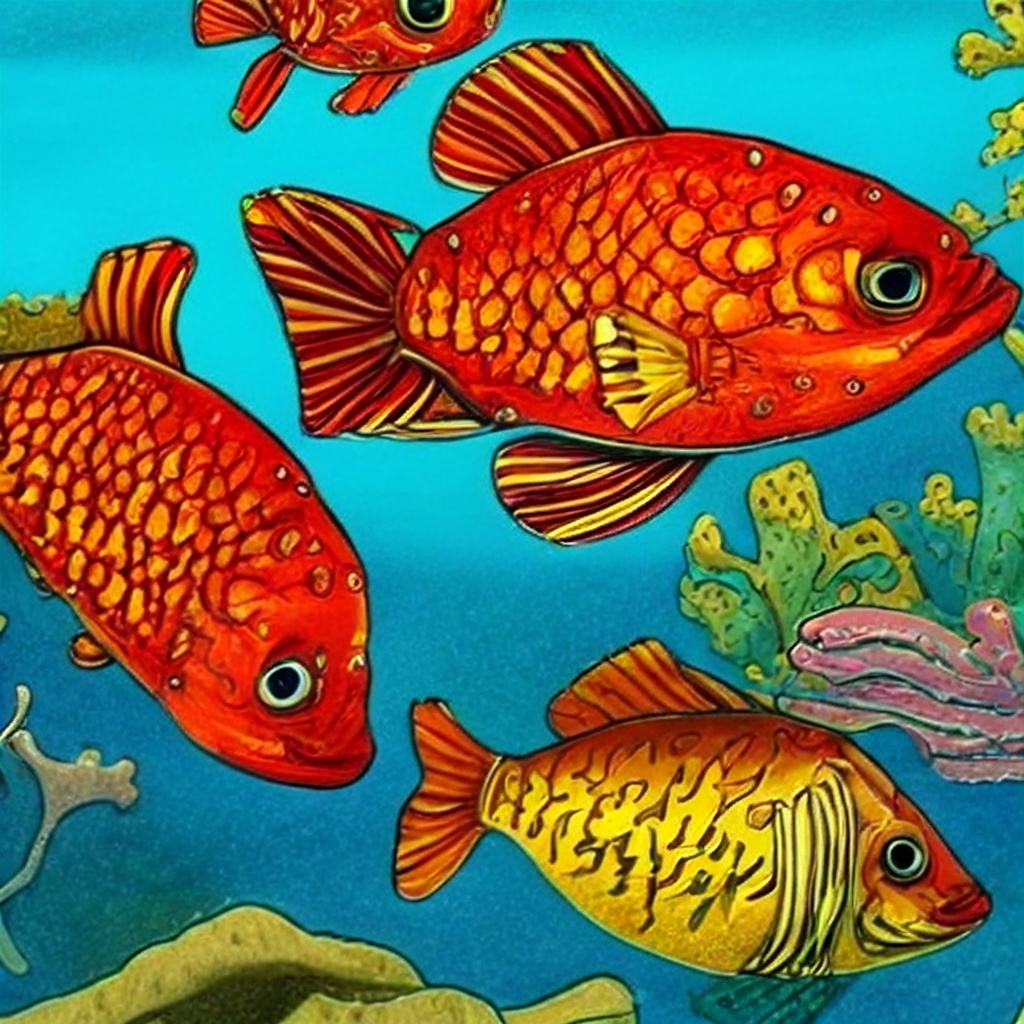
\includegraphics[width=\linewidth]{imgs/blend_source.jpg}\\{\footnotesize source}
    \end{minipage}\hfill
    \begin{minipage}{0.245\linewidth}\centering
        
\includegraphics[width=\linewidth]{imgs/blend_baseline.jpg}\\{\footnotesize hard composition}
    \end{minipage}\hfill
    \begin{minipage}{0.245\linewidth}\centering
        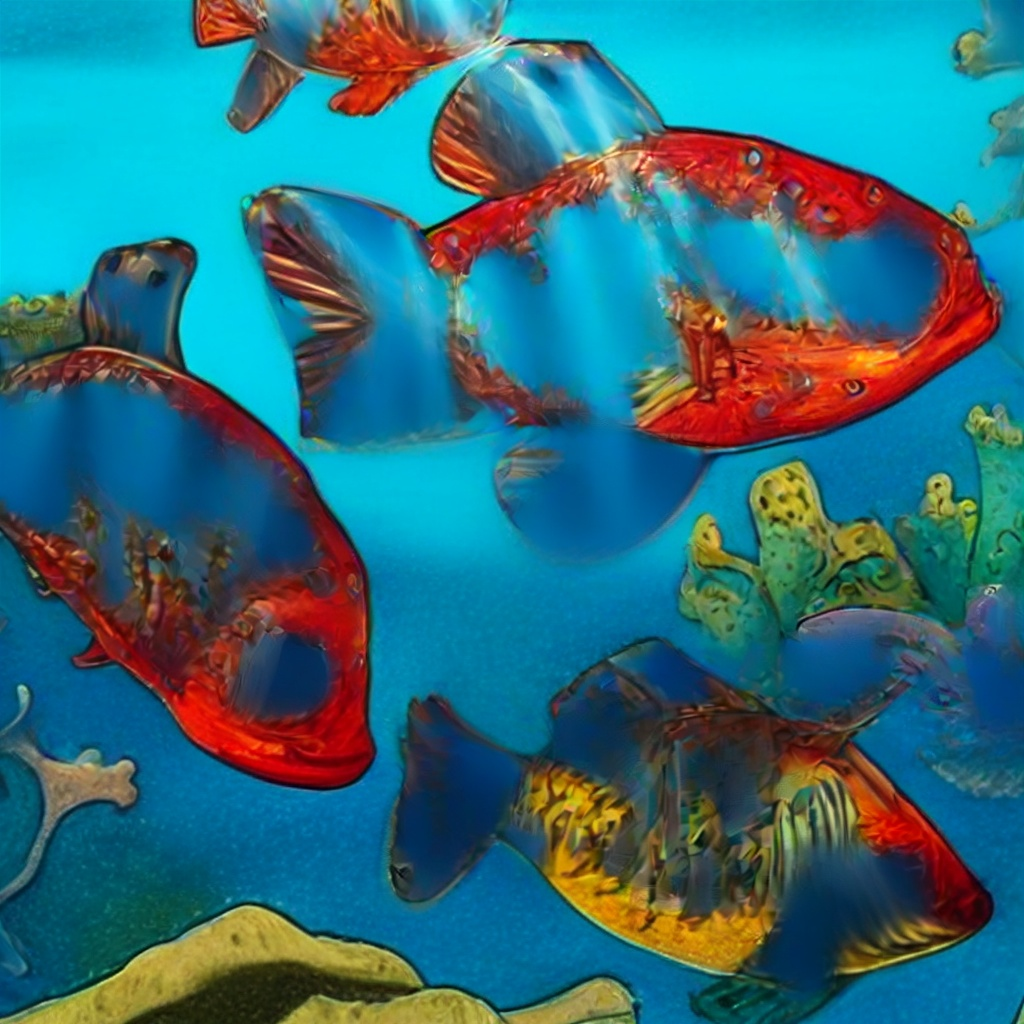
\includegraphics[width=\linewidth]{imgs/blend_hard.jpg}\\{\footnotesize blend, raw mask}
    \end{minipage}\hfill
    \begin{minipage}{0.245\linewidth}\centering
        
\includegraphics[width=\linewidth]{imgs/blend_best.jpg}\\{\footnotesize blend, cleaned mask}
    \end{minipage}
    \caption{Hard composition versus continuous blending (fish $\to$ shark). Hard composition executes the edit but drifts in style and loses much of the coral background. Blending the continuous residual at full resolution preserves both, but the last-scale attention mask is high-frequency and fragmented, so applying it directly leaves fragments of the source inside the edited region (third panel); a morphological closing and opening of the mask, a soft transition band and coarse anchoring recover the edit (fourth panel). Neither end of this axis dominates: see Sec.~\ref{sec:limitations}.}
    \label{fig:blend}
\end{figure}


% TODO(optional): promote this to a full subsection with its own table if the
% full-res blend results are included; source
% docs/new_exp/2026-07-22-fullres-blend-and-inverse-attention.md §2.

\subsection{The Threshold Is Global, Not Per Case}

A single $(h, c_{\max}, \kappa_{\max})$ is shared by every case, so the adaptation is driven only by the statistics of the attention map and not by how difficult the particular edit is. Choosing the operating point per case would require a signal that is not available before generation starts; predicting the whole metric-versus-threshold curve, or reading a signal after generation has begun, are the two natural routes and both are outside the scope of this paper.

\subsection{Dependence on Focus-Word Extraction}

Focus words are obtained by differencing the source and target prompts, which
assumes the two are structurally comparable. This assumption fails in two ways.
When the source prompt contains no anchor for the region to be edited --- most
commonly for object addition and style transfer, where the source description
simply does not mention the relevant region --- the source-side focus set is
empty and the pipeline falls back to a single-stream path. When the two prompts
are written independently and differ in phrasing rather than in content, the
difference contains words that are not edit-relevant. We quantify both cases in
Appendix~\ref{app:prompt}: on this benchmark, $230$ of $700$ source prompts yield
an empty focus set. A prompt encoder that identifies edit-relevant spans directly,
rather than by set difference, would remove the assumption entirely.
% TODO: write Appendix app:prompt from docs/reports/m14_minimal_rewrite_pipeline
% (experiments 4-5) and docs/reports/prompt_length_comparison_m15.  Keep the main
% tables free of the rewriting module: report it as an analysis of the failure
% mode plus an optional preprocessing step, not as part of the method.

\subsection{Backbone Dependence and Outlook}

Editing quality on fine textures is bounded by the reconstruction fidelity of the
backbone, and any bias of the base model propagates into the edit. The
mechanism itself, however, makes no assumption beyond next-scale prediction over
spatially localized discrete tokens with cross-modal attention. Recent extensions
of visual autoregressive modeling to video generate frames under the same
coarse-to-fine schedule, and the mask construction described here is orthogonal
to the temporal axis: the same per-scale focus and preserve masks can be built
from each frame's cross-attention and composed with the same token substitution
rule. Combined with an inference cost of about $2.5$\,s per image on a single
consumer GPU --- one to two orders of magnitude below inversion-based editors ---
this makes training-free editing of autoregressively generated video a concrete
next target rather than a speculative one.
